\chapter{Fachschaftika? Kann man das essen?}

\section{Die Fachschaft}
Wir sind die Gruppe Aktiver Fachschaftika oder kurz GAF. Ein Fachschaftikon ist ein Mitglied einer Fachschaft, das sind alle Studika eines Studiengangs, also auch du, ob du willst oder nicht. Spricht man über \emph{die Fachschaft}, meint man damit meist die aktiven Fachschaftika, die versuchen, die Uni für alle Studika lebenswerter zu machen. Die GAF ist der Zusammenschluss aus aktiven Fachschaftika der Fachbereiche Mathematik, Physik und Informatik sowie der verwandten Fächer (Medieninformatik, Wirtschaftsmathematik, Meteorologie,\ldots).

\section{Aufgaben der Fachschaft}

Was die Fachschaft tut, lässt sich grob in zwei Bereiche teilen: auf der einen Seite vertritt sie die Studika zur Seite der Fakultät hin, auf der anderen kümmert sie sich um die Studika selbst.

Durch Repräsentation in verschiedenen Gremien verleihen wir der Meinung und den Interessen der Studika Gewicht und versuchen so, Entscheidungen über die Köpfe der Studika hinweg zu unterbinden. Die wichtigsten Gremien hierfür sind:
\begin{itemize}
\item Der Fakulträtsrat (entscheidet alles wichtige innerhalb der Fakultät und ist Ort des Informationsaustausches)
\item Die Studienersatzmittelkommission (ehemals Studiengebührenkommission; beschließt, wofür Geld ausgegeben wird)
\item Die Berufungskommissionen (bestimmt, wer als neues Professorikon an unsere Uni kommt und hier auch lehrt)
\item Der Konvent der Fachschaften (besteht aus Vertretern aller Fachschaften, beschäftigt sich mit fächerübergreifenden studentischen Themen)
\end{itemize}

Unsere Aufgaben und Angebote für die Studika, also auch dich, umfassen:
\begin{itemize}
\item Altklausuren und Prüfungsprotokolle (beachte den Generationenvertrag, denn die Sammlung existiert nur, weil ältere Studika ihre Prüfungen zu uns gebracht haben, also tu dies auch für deine Nachfolger!)
\item Informationen und Beratung (O"~Phase, Ansprechpartner für Probleme, bei denen du nicht weißt, an wen du dich wenden sollst)
\item Bespaßung (Fakultätsfest, Partys und Veranstaltungen sonstiger unterhaltender Natur)
\item Unterstützung bei der Umsetzung deiner Ideen (durch tatkräftige Mitarbeit und Know How)
\end{itemize}

Wenn du dir selbst einen Eindruck von unserer Arbeit verschaffen willst, melde dich zum EWO (Ersti-Wochenende) an, komm bei uns im Büro vorbei oder auf eine Sitzung. Die Termine dafür findest du unter \ref{gaf}.

Wichtig zu wissen ist, dass wir alles das ehrenamtlich machen und das Geld, das uns zur Verfügung steht, nur zugunsten der Studika einsetzen. Der einzige Lohn unserer Arbeit ist mehr Lebenserfahrung und in manchen Fällen ein verlängertes Studium.

\begin{urlList}
	\httpsItem{gaf.fs.lmu.de}{gaf}
\end{urlList}

\section{Kontakt}\label{gafKontakt}
%XXX To do: seperate Box/ optisch aufwerten
\begin{tabular}{ l l l l }
Telefon&089 / 2180\emd{}4382\\
Telefax&089 / 2180\emd{}4391\\
&\\
&\mail{gaf@fs.lmu.de}\\
&\mail{gumbel@fs.lmu.de}\\
&\\
&\url{\https gaf.fs.lmu.de}\\
&\url{\https facebook.com/gaflmu}\\
&\\
IRC & \#gaf auf freenode
\end{tabular}

\section{Andere Fachschaften}
\begin{urlList}
	\httpsItem[Medieninformatik]{mi.fs.lmu.de}
	\httpItem[Bioinformatik]{www.bioinformatik-muenchen.com/bioinfocom/fachschaft/}
	\httpItem[Meteorologie]{www.meteo.physik.lmu.de/~studmet}
\end{urlList}

\skiptobottom
%XXX To do: neues Bild
%\centerline{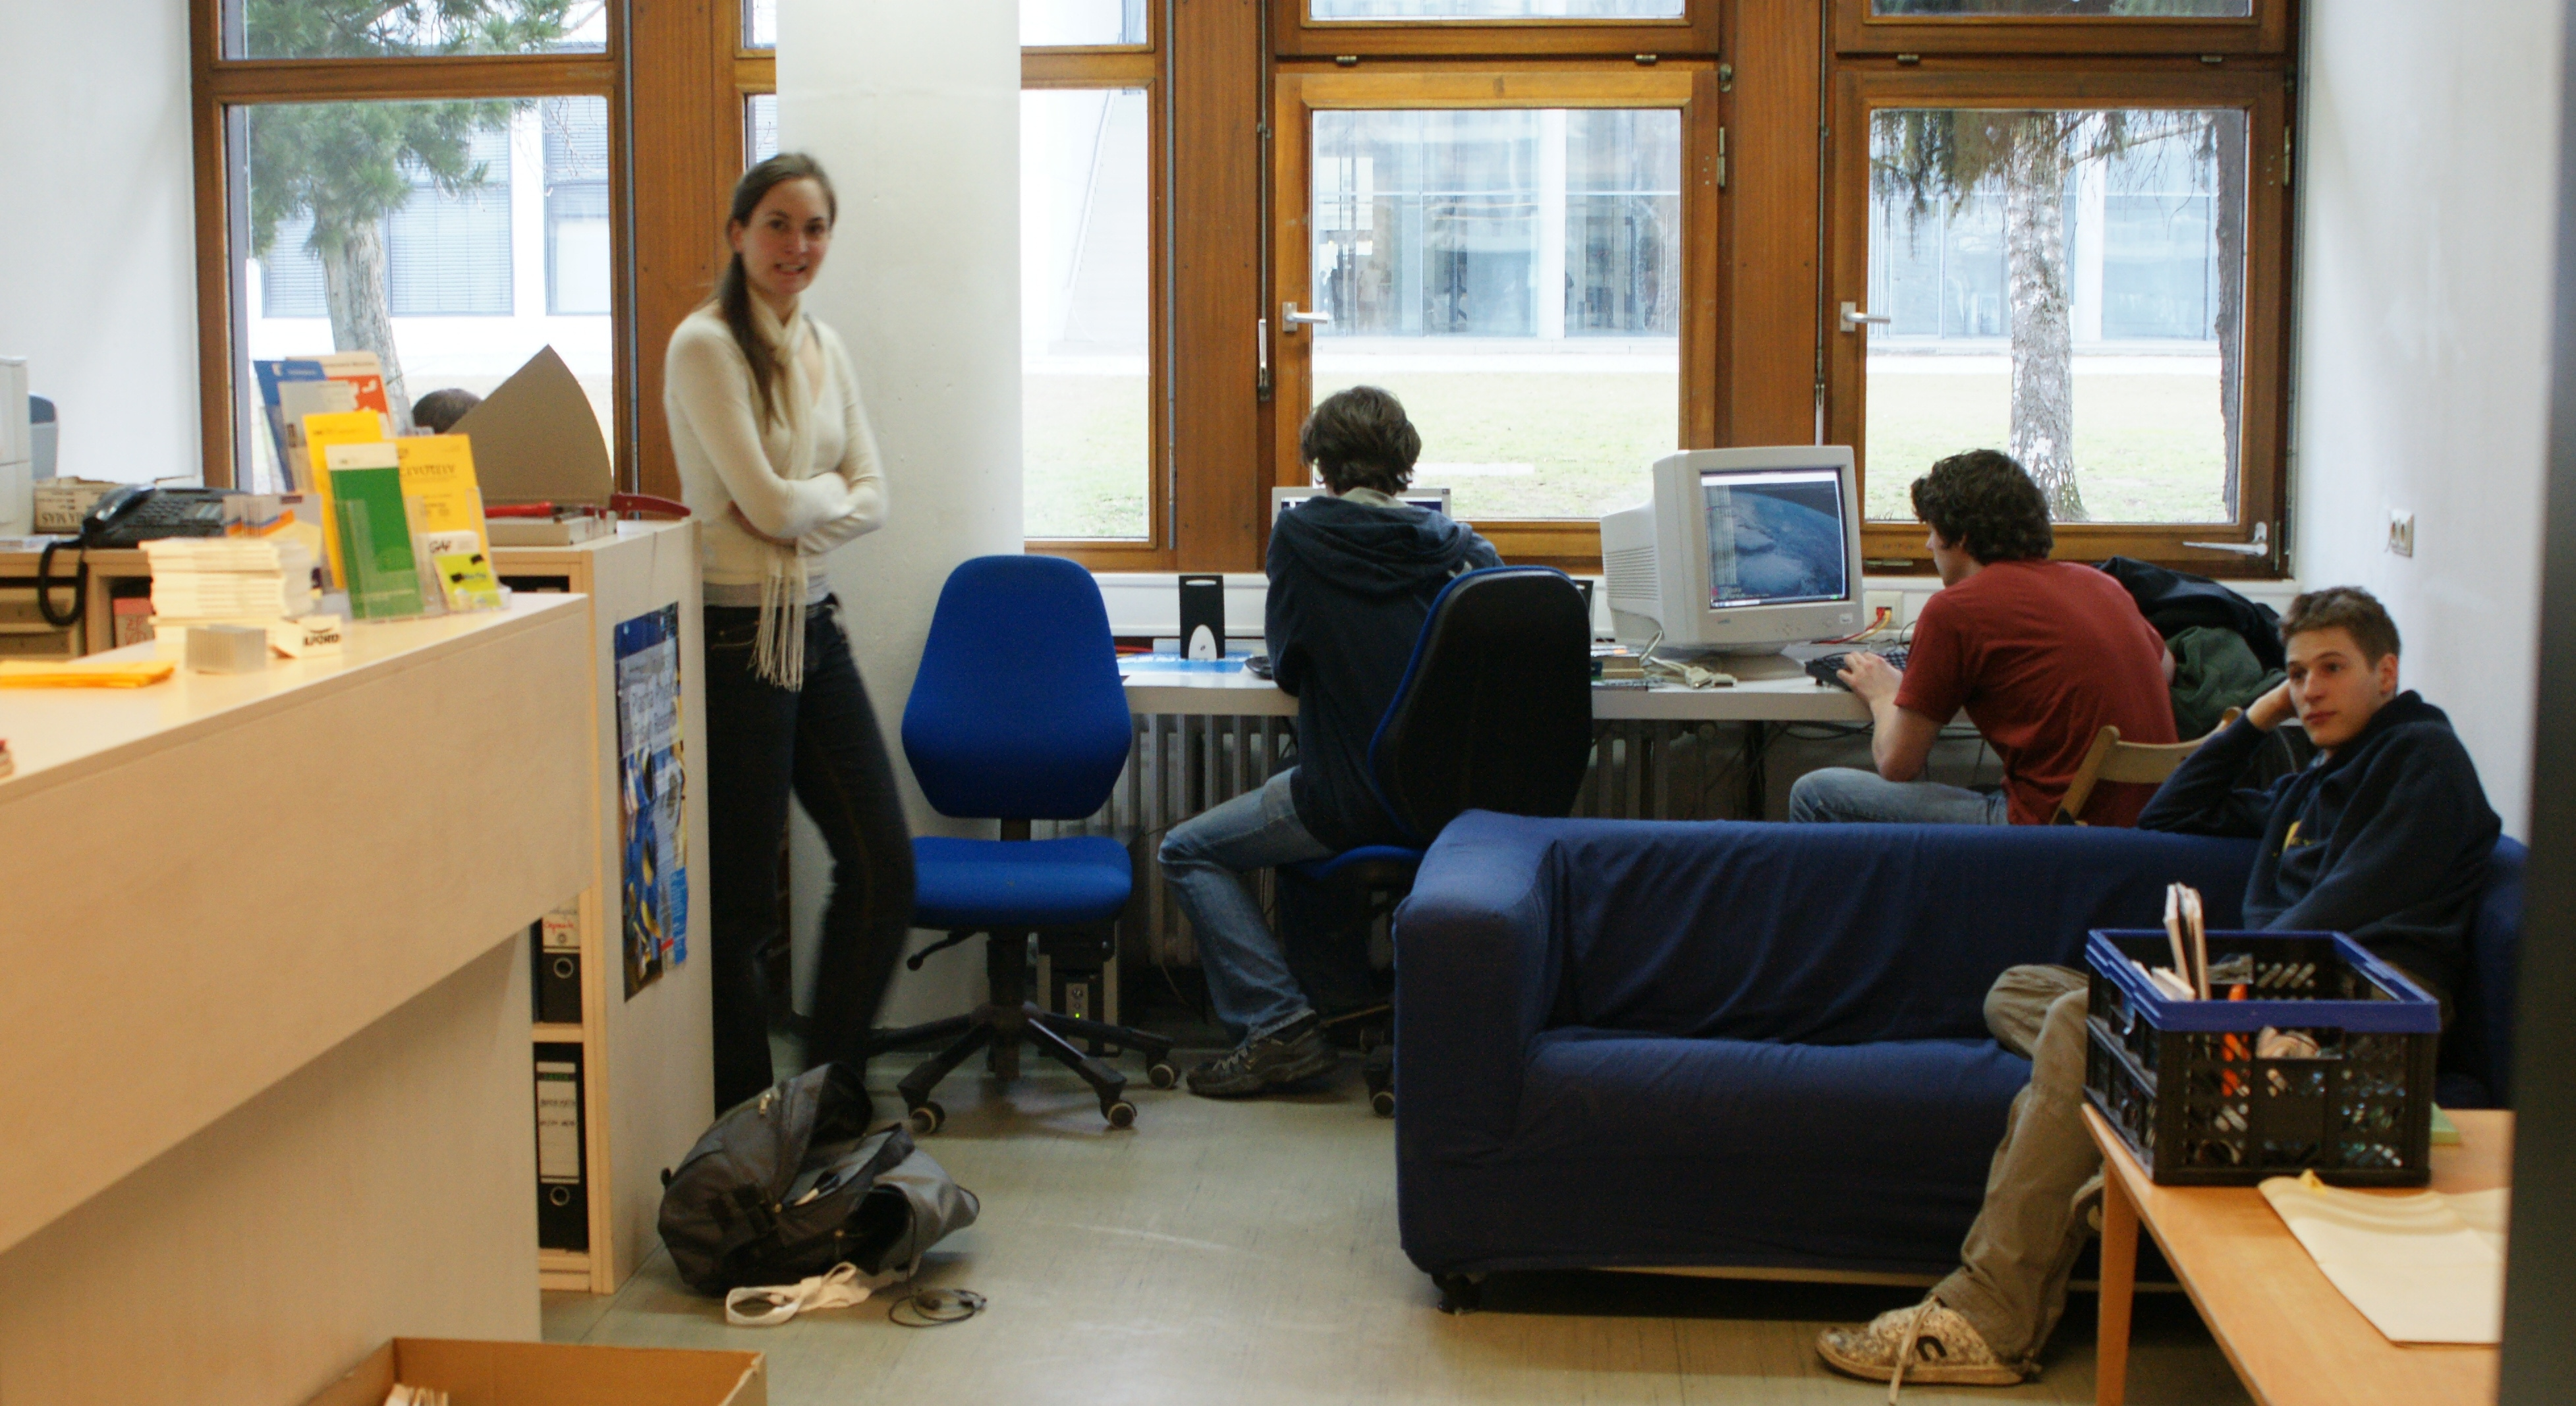
\includegraphics[width=0.8\textwidth]{aktive-fachschaft_print}}
